\chapter{Huấn luyện mạng nơ-ron nhiều tầng ẩn bằng thuật toán Adam}
\label{Chapter3}

\textit{Chương này trình bày về thuật toán tối ưu Adam và cách thuật toán khắc phục khó khăn trong huấn luyện mạng nơ-ron nhiều tầng ẩn mà khoá luận tập trung tìm hiểu. Đầu tiên chúng tôi trình bày về các thuật toán nền tảng: (1) thuật toán Gradient Descent với Momentum để tăng tốc và giảm dao động trong quá trình di chuyển trên bề mặt lỗi, và (2) thuật toán Gradient Descent với tỉ lệ học thích ứng với từng trọng số, cụ thể là thuật toán Adagrad và RMSprop. Dựa trên nền hai thuật toán này, chúng tôi trình bày ý tưởng của thuật toán Adam cũng như những ưu/khuyết điểm của thuật toán trong giải quyết các khó khăn của bài toán huấn luyện mạng nơ-ron.}

\section{Thuật toán Gradient Descent với Momentum}

Các thuật toán sử dụng gradient như GD và SGD gặp phải hai khó khăn chính khi thiếu đi thông tin về độ cong của bề mặt lỗi. Đầu tiên, vì hướng của gradient là hướng có độ dốc lớn nhất nên không phải lúc nào cũng là hướng tốt nhất và có thể gây dao động mạnh trong khi độ lỗi giảm không nhiều. Thứ hai, ``độ nhạy cảm'' của mỗi trọng số là khác nhau trong bề mặt lỗi, vì vậy áp dụng một tỷ lệ học chung cho tất cả các trọng số sẽ khiến cho hướng cập nhật bỏ qua các trọng số có ``độ nhạy cảm'' nhỏ.

``GD/SGD với Momentum'' (hay ``Momentum'') là một phương pháp cải tiến sử dụng quán tính để điều chỉnh hướng gradient theo hướng tốt nhất về cực tiểu, từ đó tăng tốc độ di chuyển trên bề mặt lỗi. Quán tính được thêm vào công thức thông qua hệ số quán tính $\beta$. Tại mỗi bước $t$, véc-tơ quán tính $m_t$ được xác định bởi công thức \ref{eqn:mt}:

\begin{equation}
	\label{eqn:mt}
	m_t = \beta m_{t-1} + \eta\nabla_\theta E(\theta_t)
\end{equation}
với $m_{t-1}$ là véc-tơ quán tính trước đó, $\eta$ là tỉ lệ học và $\nabla_\theta E(\theta_t)$ là gradient của hàm chi phí tại $\theta_t$.

Từ công thức \ref{eqn:mt} ta có công thức cập nhật $\theta$ tại mỗi bước được cải tiến như sau:

\begin{equation}
	\label{eqn:theta-momentum}
	\theta_t = \theta_{t-1} - v_t
\end{equation}

Nhờ vào sự cải tiến đơn giản này mà thuật toán Momentum có thể giảm bớt sự di chuyển tại những hướng mà dấu của gradient không ổn định, đồng thời tăng cường sự di chuyển tại hướng mà dấu của gradient ổn định. Mức độ điều chỉnh sự di chuyển phụ thuộc vào hệ số quán tính $\beta$. Một hệ số $\beta$ quá lớn cũng như quá nhỏ đều kéo dài thời gian huấn luyện của mô hình. Nếu $\beta$ được chọn quá lớn thì mức độ thay đổi quá lớn dẫn đến thuật toán bị dao động quanh điểm cực tiểu; nếu $\beta$ chọn quá nhỏ, thuật toán Momentum sẽ suy biến về GD và khó khăn sẽ không được khắc phục.

Có thể nói hệ số quán tính cho phép thuật toán ưu tiên các giá trị quán tính gần hơn các giá trị quán tính cũ nhờ vào đường trung bình động hàm mũ (Exponential Moving Averages) hay EMA. Đường trung bình động hàm mũ cho phép ta sử dụng trung bình động để xử lý nhiễu trong dữ liệu mà ta quan sát được và xấp xỉ nó gần hơn với dữ liệu thực. Ta thực hiện lấy trung bình trên $\frac{1}{1-\beta}$ bước nhảy gần nhất và cập nhật trọng số. Ta khai triển công thức \ref{eqn:mt} như sau:

\begin{equation}
	\label{eqn:m3}
	\begin{aligned}
		m_1 &= \beta m_0 + \eta\nabla_\theta E(\theta_1) \\ m_2 &= \beta m_1 + \eta \nabla_\theta E(\theta_2) = \beta (m_0 + \eta\nabla_\theta E(\theta_1)) + \eta\nabla_\theta E(\theta_2) \\ &= \beta m_0 + \beta\eta\nabla_\theta E(\theta_1) + \eta\nabla_\theta E(\theta_2) \\ m_3 &= \beta m_2 + \eta\nabla_\theta E(\theta_3) = \beta (\beta m_0 + \beta\eta\nabla_\theta E(\theta_1) + \eta\nabla_\theta E(\theta_2)) + \eta\nabla_\theta E(\theta_3) \\ &= \beta^2 m_0 + \beta^2\eta \nabla_\theta E(\theta_1) + \beta \eta \nabla_\theta E(\theta_2) +\eta \nabla_\theta E(\theta_3)
	\end{aligned}
\end{equation}

Từ công thức \ref{eqn:m3} ta nhận thấy rằng tại bước nhảy thứ $t$, giá trị của momentum phụ thuộc vào các giá trị momentum trước đó từ $1..(t-1)$. Mỗi giá trị trong dãy đều được nhân với hệ số $\beta ^t$. Vì $\beta$ là hệ số quán tính nằm trong khoảng $(0,1)$ nên $\beta^t$ sẽ càng nhỏ khi $t$ càng lớn dẫn đến các giá trị càng lâu trước đó sẽ có hệ số càng nhỏ và dần không đóng góp gì nhiều trong quá trình huấn luyện. Hay nói cách khác, các giá trị này dần được quên đi và thuật toán Momentum quan tâm nhiều đến các giá trị gần với hiện tại.

Trong thực tế huấn luyện, ta thường sử dụng cách xấp xỉ true gradient bằng các gradient của tập con để tăng tốc quá trình cập nhật trọng số. Trong quá trình xấp xỉ, việc tạo minibatch bằng cách gom nhóm ngẫu nhiên các điểm dữ liệu đã thêm một lượng nhiễu vào trong quá trình tối ưu. So sánh độ lớn của nhiễu với độ lớn của momentum ta có thể chia quá trình thành hai giai đoạn: giai đoạn ``transient'' và giai đoạn ``fine-tuning''. Trong giai đoạn transient, momentum vẫn còn hiệu quả trong điều chỉnh hướng của gradient và giúp gradient tiến nhanh về vị trí có cực tiểu vì độ lớn của momentum lớn hơn độ lớn của nhiễu. Quá trình huấn luyện càng lâu, độ lớn của momentum ngày càng giảm và bị lấn át bởi độ nhiễu, khi đó ta bước qua giai đoạn fine-tuning. Trong các mạng nơ-ron nhiều tầng ẩn, giai đoạn fine-tuning chiếm một phần ít hơn và cũng ít quan trọng hơn giai đoạn transient nên việc đảm bảo giai đoạn transient được diễn ra đủ lâu là một sự cần thiết \cite{sutskever2013onti}.

Sự chuyển đổi giữa hai quá trình được kể trên được quyết định bởi hằng số quán tính $\beta$. Sử dụng một hệ số quán tính $\beta$ lớn cho phép momentum thực hiện quá trình tối ưu tốt hơn trên các hướng có ``độ nhạy cảm'' nhỏ. Tuy nhiên, lợi thế này không được thể hiện qua rõ ràng qua độ lỗi do thuật toán không thể hội tụ tốt tại các hướng có ``độ nhạy cảm'' cao với một hệ số quán tính $\beta$ lớn. Sự đánh đổi này cho kết quả là ta có thể tiến gần đến vùng có cực tiểu hoặc là hội tụ tại cực tiểu có độ lỗi nhỏ hơn. Trong khi sử dụng một hệ số $\beta$ nhỏ sẽ cho độ lỗi cao hơn vì giai đoạn transient kết thúc quá sớm. Thiếu đi sự hỗ trợ của momentum, các phương pháp bậc nhất không thể tận dụng tốt thông tin tại các hướng có ``độ nhạy cảm'' nhỏ và rất dễ bỏ qua các vùng chứa cực tiểu hoặc cực tiểu có độ lỗi thấp hơn dẫn đến hội tụ tại điểm có độ lỗi cao.

\begin{figure}[htp]
	\centering
	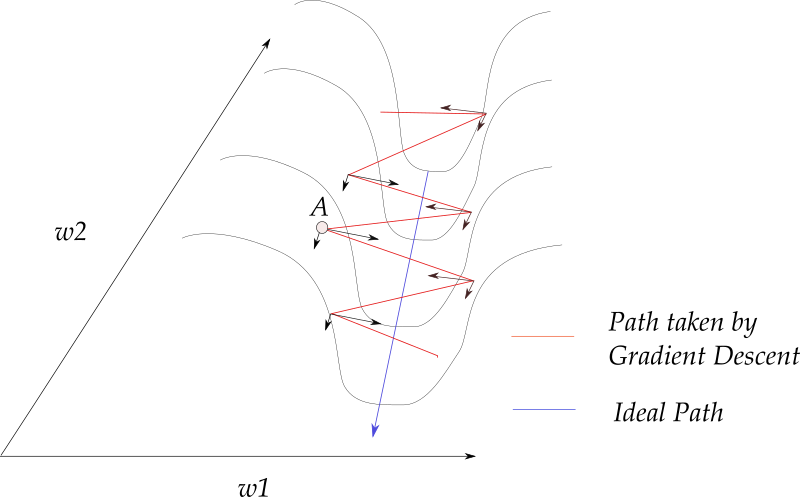
\includegraphics[width=140 mm]{images/valley-momentum.png}
	\caption{Minh họa cách Momentum triệt tiêu hướng có độ dốc lớn. (Nguồn: \url{https://blog.paperspace.com/intro-to-optimization-momentum-rmsprop-adam/})}
	\label{fig:valley-momentum}
\end{figure}

Hình \ref{fig:valley-momentum} mô tả một rãnh hẹp trong không gian hai chiều có trục tung là $w_2$ và trục hoành là $w_1$. Các rãnh hẹp này thường được hình thành do sự khác biệt giữa các giá trị trọng số do độ quan trọng của giá trị đầu ra của mỗi nơ-ron khác nhau là khác nhau. Các liên kết đến nơ-ron lưu trữ đặc trưng quan trọng ảnh hướng đến dự đoán của mạng nơ-ron thường được gán giá trị trọng số lớn hơn các nơ-ron mang ít thông tin. Giả sử ta gán $w_1 = 10$ và $w_2 = 1$ thì tín hiệu của nơ-ron được liên kết bằng $w_1$ sẽ ảnh hưởng lên độ lỗi gấp 10 lần tín hiệu của nơ-ron được liên kết bằng $w_2$ dẫn đến độ cong ở hướng $w_1$ cao hơn hướng $w_2$ và tạo thành một rãnh hẹp.

Trong địa hình rãnh hẹp, ta mong muốn bước một bước nhỏ theo hướng có độ cong cao và một bước dài theo hướng có độ cong thấp, bằng phẳng hơn. Tuy nhiên, công thức bước cập nhật của thuật toán GD (công thức \ref{eqn:theta-batch-update}) cho ta điều ngược lại. Kết quả là thời gian huấn luyện kéo dài nhưng độ lỗi giảm không đáng kể do thuật toán bị dao động tại hướng có độ dốc cao và chỉ đi những bước nhỏ tại hướng tối ưu có độ dốc thấp (hình \ref{fig:valley-momentum}). Một giải pháp thường được sử dụng để khắc phục hiện tượng này là giảm tỉ lệ học của thuật toán GD/SGD. Tuy nhiên, với một tỉ lệ học nhỏ, thuật toán GD/SGD không thể "khám phá" những hướng có độ dốc nhỏ một cách hiệu quả do độ lớn bước cập nhật tại những hướng này là rất nhỏ và dễ dàng bị lấn át bởi hướng có độ dốc cao. Trong trường hợp hướng đi về cực tiểu là một trong các hướng có độ dốc thấp, thuật toán GD/SGD sẽ cho độ lỗi giảm rất chậm tạo cảm giác huấn luyện bị chững lại như gặp phải cực tiểu địa phương.

\begin{figure}[htp]
	\centering
	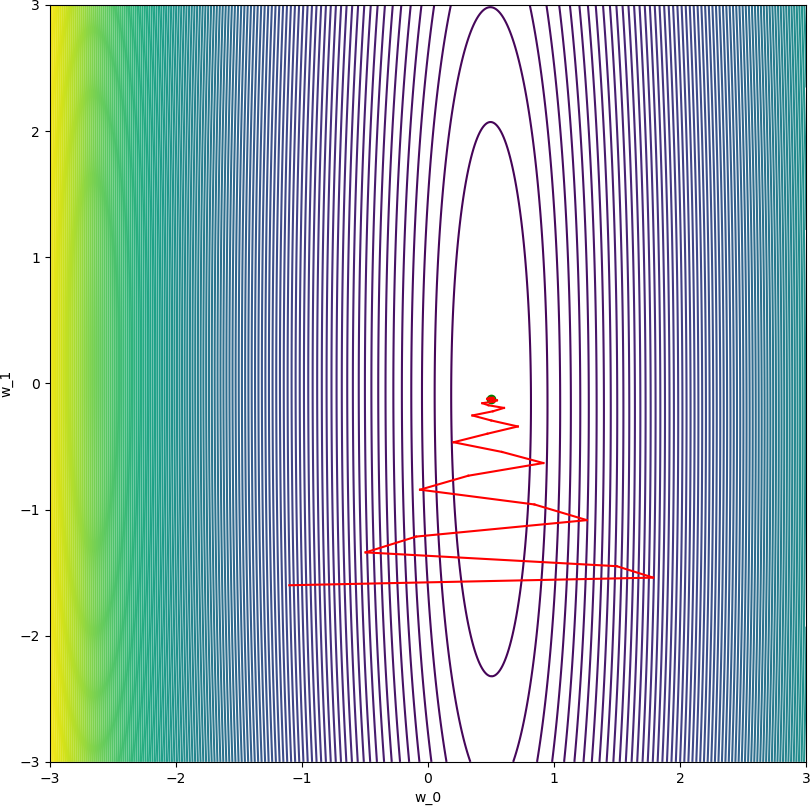
\includegraphics[width=85 mm]{images/gdm.png}
	\caption{Mô tả đường đi của thuật toán GD khi có thêm lượng quán tính trong rãnh hẹp.}
	\label{fig:gd-m}
\end{figure}

Momentum giúp giải quyết vấn đề này bằng cách sử dụng gradient tại điểm hiện tại và các giá trị gradient gần trong quá khứ. Trong rãnh hẹp được mô tả như trong hình \ref{fig:valley-momentum}, ta lấy một điểm $A$ bất kỳ. Tại đó, ta luôn có thể phân tích thành hai véc-tơ đạo hảm riêng tương ứng với từng hướng $w_1$ và $w_2$. Vì hướng $w_1$ có độ cong cao hơn hướng $w_2$ nên véc-tơ đạo hàm riêng tại hướng $w_1$ sẽ dài hơn hướng $w_2$. Ta có thể dễ dàng nhận thấy chiều véc-tơ đạo hàm riêng theo hướng $w_1$ thay đổi liên tục tại từng bước cập nhật trong khi véc-tơ đạo hàm riêng theo hướng $w_2$ ổn định qua nhiều bước liên tiếp. Sự thay đổi chiều liên tục đồng nghĩa với việc dấu của giá trị đạo hàm riêng cũng thay đổi liên tục. Do đó, khi thuật toán Momentum tíến hành cộng dồn các giá trị gradient thì các véc-tơ đạo hàm riêng thành phần tại hướng có độ dốc cao như $w_1$ sẽ bị triệt tiêu và ngược lại các véc-tơ thành phần tại các hướng như $w_2$ sẽ được tăng cường. Vì vậy, thuật toán cho phép hạn chế sự di chuyển tại hướng có dấu của gradient không ổn định và tăng cường sự di chuyển tại hướng mà dấu của gradient ổn định. Từ đó mà lượng ``quán tính'' được thêm vào trong các bước cập nhật giúp điều chỉnh hướng cập nhật và tăng tốc quá trình di chuyển trong vùng rãnh hẹp.

Đường đi của hai thuật toán GD và SGD khi có thêm momentum chứng thực cho lý thuyết trên. Hình \ref{fig:gd-m} cho ta đường đi của thuật toán GD có thêm momentum trong rãnh hẹp. Qua đó ta thấy được rằng đường đi ít dao động, và các bước nhảy tiến nhanh về phía cực tiểu hơn khi sử dụng thuật toán GD thuần tuý (Hình \ref{fig:gd-sgd}a). Điều tương tự cũng xảy ra với thuật toán SGD. Hình \ref{fig:sgd-m} mô tả đường đi của thuật toán SGD khi có thêm lượng momentum trong vùng rãnh hẹp. Ta có thể dễ dàng nhận ra hai giai đoạn của huấn luyện được đề cập ở phần lý thuyết. Trong giai đoạn transient, thuật toán di chuyển nhanh và không xảy ra hiện tượng dao động nhiều ở vùng rãnh hẹp. Đồng thời độ lỗi cũng giảm đáng kể sau một lần cập nhật và độ nhiễu đến từ việc gom nhóm ngẫu nhiên dữ liệu cũng được hạn chế hơn so với hình \ref{fig:gd-sgd}b. Tuy nhiên, càng về sau, khi bước qua giai đoạn finetuning, thì đường đi ngày càng nhiều dao động là minh chứng cho phần momentum bị độ nhiễu lấn át và thuật toán suy biến về SGD thuần tuý.

\begin{figure}[htp]
	\centering
	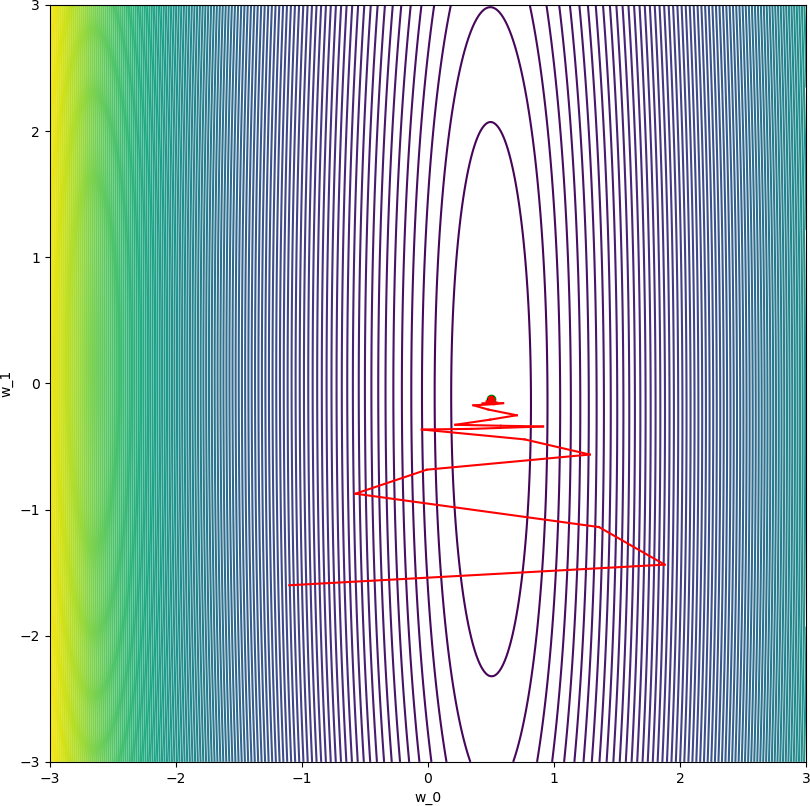
\includegraphics[width=85 mm]{images/sgdm.png}
	\caption{Mô tả đường đi của thuật toán SGD khi có thêm lượng quán tính trong rãnh hẹp.}
	\label{fig:sgd-m}
\end{figure}

Tuy nhiên, trong các vùng mà cách biệt độ lớn giữa các giá trị trọng số là rất lớn, thuật toán Momentum vẫn còn gặp những hạn chế do không có khả năng điều chỉnh tỉ lệ học thích ứng theo từng hướng. Thêm nữa, Richard S. Sutton cho rằng mặc dù thuật toán Momentum tăng tốc quá trình huấn luyện, nhưng lượng tăng tốc này vẫn còn khá nhỏ \cite{sutton1986two}. Đồng thời, bài báo cũng cho rằng để thực hiện một bước nhảy tối ưu, ta cần điều chỉnh tỷ lệ học nhỏ tại những hướng có độ cong cao và sử dụng một tỷ lệ học lớn hơn tại những hướng có độ cong thấp hơn. Đây cũng chính là ý tưởng của các phương pháp tỉ lệ học thích ứng.

\section{Thuật toán Gradient Descent với tỉ lệ học thích ứng}

Việc dự đoán trong học máy nói chung và mạng nơ-ron nhiều tầng ẩn nói riêng dựa vào quá trình trích xuất và liên hệ các đặc trưng của dữ liệu. Thông thường, các điểm dữ liệu trong cùng một bài toán sẽ có những đặc trưng chung thường gặp. Tuy nhiên, cũng có một số đặc trưng rất hiếm khi xuất hiện, chỉ có ở trong một số ít điểm dữ liệu cụ thể. Các đặc trưng hiếm gặp này thường sẽ có ảnh hưởng rất lớn về mặt ý nghĩa của dữ liệu, và mang lại rất nhiều thông tin về điểm dữ liệu đó\cite{salton1988term}. Một ví dụ cụ thể là trong phân tích văn bản, các từ xuất hiện thường xuyên như các liên từ (``và'', ``thì'', ``nhưng'',...) hay các phó từ (``cũng'', ``lại'', ``rồi'',...) lại không thể hiện nội dung nhiều bằng các danh từ và động từ chỉ các đối tượng, hành động cụ thể. Một trường hợp khác là khi xét riêng một đặc trưng, những điểm dữ liệu mang giá trị khác với các điểm dữ liệu còn lại đóng vai trò quan trọng hơn trong việc cung cấp thông tin để giải quyết bài toán.

Tuy nhiên, các thông tin quan trọng được biểu diễn bằng các đặc trưng hiếm lại ít được mạng nơ-ron nhiều tầng ẩn chú ý. Trong mạng nơ-ron nhiều tầng ẩn, các nơ-ron tương ứng với các đặc trưng thường gặp sẽ được cập nhật thường xuyên, trong khi các nơ-ron tương ứng với các đặc trưng hiếm chỉ được cập nhật một số ít lần trong một lần duyệt qua toàn tập dữ liệu. Hiện tượng này khiến cho các đặc trưng thường gặp và mang ít thông tin được biểu diễn tốt hơn, còn các đặc trưng hiếm mang nhiều ý nghĩa lại chưa được học.

Mặc dù SGD và Momentum thực hiện cập nhật một lượng khác nhau cho mỗi trọng số tùy theo độ lớn của gradient tại điểm đang xét (và trạng thái của momentum tại thời điểm đó), tuy nhiên lượng cập nhật vẫn chỉ dựa vào hướng và độ dốc của gradient, hay nói cách khác là độ dốc của bề mặt lỗi, tại điểm đang xét và chưa tính tới độ nhạy cảm của các trọng số. John Duchi, Elad Hazan, và Yoram Singer đã đề xuất thuật toán Adagrad\cite{duchi2011adaptive} lấy ý tưởng từ phương pháp Newton để giải quyết vấn đề này bằng cách thích ứng lượng cập nhật cho từng trọng số: các trọng số tương ứng với các đặc trưng thường gặp sẽ được cập nhật ít hơn, còn các trọng số tương ứng với các đặc trưng hiếm sẽ được cập nhật lượng lớn hơn.

\begin{itemize}
	\item Từ khai triển Taylor ở công thức \ref{eqn:taylor-f}, chúng ta có thể tạo được một xấp xỉ bậc hai $\rho$ của hàm $f$ cho các giá trị $x$ xung quanh một điểm $x_0$:
	\begin{equation}
		\label{eqn:quad-approx}
		f(x) \approx \rho(x) = f(x_0) + f'(x_0) \cdot (x - x_0) + \frac{1}{2} \cdot f''(x_0) \cdot (x - x_0)^2
	\end{equation}
	\begin{figure}[H]
		\centering
		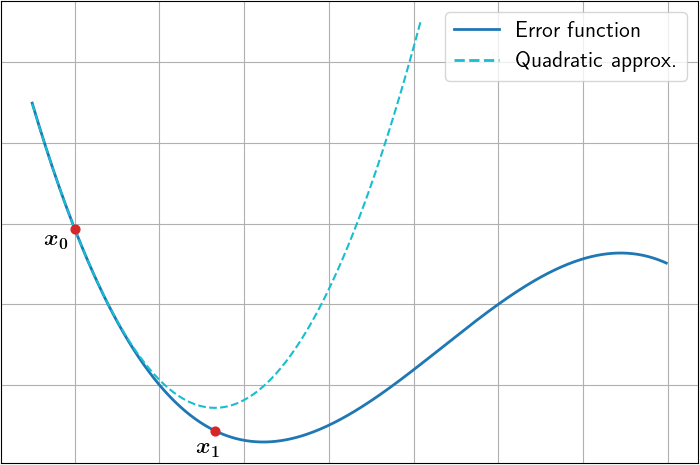
\includegraphics[width=120 mm]{images/quad-approx.png}
		\caption{Xấp xỉ bậc hai (đường đứt khúc màu xanh nhạt) của hàm lỗi (đường màu xanh đậm) và bước cập nhật tiếp theo của phương pháp Newton.}
		\label{fig:newton-step}
	\end{figure}
	Vì đây là một xấp xỉ bậc hai nên chúng ta có thể tìm cực trị của xấp xỉ này bằng cách giải phương trình $\rho '(x) = 0$. Khi đó nghiệm của $\rho'(x)$ sẽ là bước cập nhật tiếp theo của phương pháp Newton (hình~\ref{fig:newton-step}) được tính bằng công thức \ref{eqn:newton-update}:
	\begin{equation} \label{eqn:newton-update}
		\begin{aligned}
			\rho'(x_{t+1}) &= 0 \\
			\Rightarrow f'(x_t) + f''(x_t) \cdot (x_{t+1} - x_t) &= 0 \\
			\Rightarrow x_{t+1} &= x_t - \frac{f'(x_t)}{f''(x_t)}
		\end{aligned}
	\end{equation}

	\item Ma trận Hessian là ma trận vuông gồm các đạo hàm bậc hai theo từng cặp hướng của một hàm số. Cho một hàm số $f$ có tham số đầu vào là một véc-tơ $x \in \mathbb{R}^M$, chúng ta sẽ có ma trận vuông Hessian $H$ kích thước $M\times M$ theo công thức:
	\begin{equation}
		H = \begin{bmatrix}
			\frac{\delta^2 f}{\delta x^{2}_1} & \frac{\delta^2 f}{\delta x_1 \delta x_2} & \dotsb & \frac{\delta^2 f}{\delta x_1 \delta x_M} \\
			\frac{\delta^2 f}{\delta x_2 \delta x_1} & \frac{\delta^2 f}{\delta x^{2}_2} & \dotsb & \frac{\delta^2 f}{\delta x_2 \delta x_M} \\
			\vdots & \vdots & \ddots & \vdots \\
			\frac{\delta^2 f}{\delta x_M \delta x_1} & \frac{\delta^2 f}{\delta x_M \delta x_2} & \dotsb & \frac{\delta^2 f}{\delta x^{2}_M}
		\end{bmatrix}
	\end{equation}

	\item Để khái quát hóa phương pháp Newton cho bài toán tối ưu trong không gian cao chiều, ta thay đạo hàm bậc nhất và đạo hàm bậc hai từ công thức \ref{eqn:quad-approx} lần lượt bằng gradient $g(x_0)$ và ma trận Hessian $H$ tại điểm $x_0$:
	\begin{equation} \label{eqn:hessian-approx}
		f(x) \approx \rho(x) = f(x_0) + g(x_0)^\top (x - x_0) + \frac{1}{2}(x - x_0)^\top H(x - x_0)
	\end{equation}
	Tương tự như trên, chúng ta cũng giải phương trình $\nabla\rho(x)=0$ để tìm bước cập nhật tiếp theo:
	\begin{equation} \label{eqn:hessian-update}
		\begin{aligned}
			\nabla \rho(x_t) &= 0 \\
			\Rightarrow g(x_t) + H_t \cdot (x_{t+1} - x_t) &= 0 \\
			\Rightarrow x_{t+1} &= x_t - H^{-1}_t \cdot g(x_t)
		\end{aligned}
	\end{equation}
\end{itemize}

Tại mỗi bước cập nhật, phương pháp Newton xấp xỉ bề mặt lỗi xung quanh điểm hiện tại bằng một parabol $P$ có cùng độ dốc và độ cong với bề mặt lỗi tại điểm đang xét. Từ đó, bước cập nhật trong công thức \ref{eqn:hessian-update} sẽ cho một điểm mới là điểm cực trị trong parabol $P$ (cực tiểu nếu parabol $P$ có bề lõm quay lên trên; cực tiểu nếu parabol $P$ có bề lõm quay xuống dưới). Ví dụ một hàm số bậc hai có dạng $y_1 = ax^2 + bx + c$ sẽ có đồ thị là một parabol $P_1$ có bề lõm hướng lên và điểm cực tiểu là điểm $A(\frac{-b}{2a};\frac{-\Delta}{4a})$. Lấy một điểm B bất kỳ thuộc parabol $P_1$ có toạ độ $(x_B,y_B)$ với $x_B > \frac{-b}{2a}$. Để từ $B$ đến được cực tiểu $A$ trong một bước, thì tạo độ điểm $B$ phải thay đổi một lượng $\Delta x = x_B - x_A = x_B + \frac{b}{2a} = \frac{2ax_B + b}{2a} = \frac{f'(x_B)}{f''(x_B)}$. Vậy từ điểm $B$ ta thực hiện bước cập nhật $x_B - \Delta x$ thì ta đến được điểm $A$. Trong trường hợp hàm nhiều biến, đạo hàm bậc nhất $f'(x_B)$ sẽ được thay bằng véc-tơ gradient và đạo hàm bậc hai sẽ được thay bằng ma trận Hessian. Viết lại theo dạng tổng quát ta sẽ được công thức \ref{eqn:hessian-update}. Vì vậy các thuật toán bậc hai bị "thu hút" bởi các điểm cực trị dẫn đến mắc kẹt tại điểm yên ngựa. Đồng thời đây là một trong những lý do quan trọng khiến các phương pháp bậc hai ít được sử dụng hơn các phương pháp bậc nhất trong huấn luyện mạng nơ-ron nhiều tầng ẩn. Các phương pháp bậc nhất không gặp vấn đề này do hướng của gradient là hướng có độ thay đổi lớn nhất, đồng nghĩa với việc hướng gradient luôn chỉ về cực đại. Bằng cách đi ngược lại với hướng của gradient, ta luôn có thể tìm về một điểm mới có độ lỗi nhỏ hơn điểm hiện tại. Vấn đề của các phương pháp bậc nhất gặp phải là độ lớn bước cập nhật quá nhỏ. Các phương pháp tỉ lệ học thích ứng giúp thay đổi điều này bằng thông tin xấp xỉ được từ ma trận Hessian để thay đổi kích thước của bước cập nhật.

Ngoài ra, phương pháp Newton phụ thuộc khá lớn vào việc xấp xỉ cục bộ tại một điểm trên bề mặt lỗi. Vì vậy, một xấp xỉ không chính xác dễ dàng gây ra những bước cập nhật kém hiệu quả và có khả năng thuật toán không thể hội tụ tại cực tiểu. Các trường hợp này thường xảy ra khi các đạo hàm riêng bậc hai bằng 0 hoặc tiến gần về 0, khiến cho việc xấp xỉ bằng ma trận nghịch đảo không còn chính xác. Từ đó công thức \ref{eqn:hessian-update} cho ta một điểm mới có độ lỗi lớn hơn điểm hiện tại (hình \ref{fig:newton-bad-step}).

\begin{figure}
	\centering
	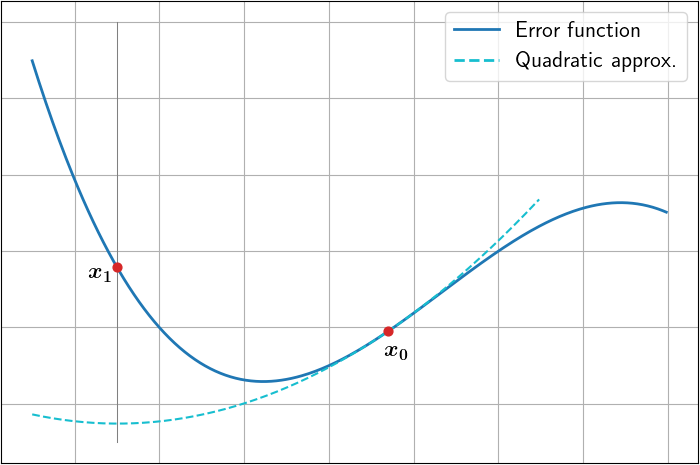
\includegraphics[width=120 mm]{images/hessian-osc.png}
	\caption{Cực tiểu của xấp xỉ bậc hai cung cấp một bước cập nhật không tối ưu.}
	\label{fig:newton-bad-step}
\end{figure}

Một hạn chế khác của các phương pháp bậc hai như phương pháp Newton nằm ở việc tính toán ma trận Hessian. Trong không gian $\mathbb{R}^M$ với $M$ có thể lên tới hàng trăm triệu hay thậm chí là hàng tỷ tương ứng với số trọng số của mô hình, ma trận Hessian sẽ yêu cầu thời gian tính toán và bộ nhớ quá lớn, dẫn đến việc sử dụng các phương pháp bậc hai cho bài toán tối ưu mạng nơ-ron nhiều tầng ẩn là bất khả thi.

Thuật toán Adagrad cũng sử dụng nguyên lý xấp xỉ bề mặt lỗi tương tự như phương pháp Newton. Tuy nhiên, thay vì tính trực tiếp ma trận Hessian nghịch đảo ($H^{-1}$, công thức \ref{eqn:hessian-update}), Adagrad chỉ thực hiện xấp xỉ tương đối $H^{-1}$ và tính bước cập nhật tiếp theo bằng công thức \ref{eqn:adagrad-base}:

\begin{equation}
	\label{eqn:adagrad-base}
	x_{t+1} = \prod^{diag(G_t)^{1/2}}_{X}(x_t-\eta\cdot diag(G_t)^{-1/2}\cdot g_t)
\end{equation}
với $g_t$ là véc-tơ gradient ở thời điểm $t$ và $G_t = \sum^{t}_{i=0}g_i\cdot g^{\top}_i$. Công thức \ref{eqn:adagrad-base} chỉ sử dụng gradient bậc nhất để xấp xỉ đường chéo của ma trận Hessian. Vì các bước tính đường chéo và căn bậc hai của ma trận $G_t$ có chi phí tuyến tính nên thuật toán Adagrad vẫn đảm bảo hiệu quả tính toán.

\begin{itemize}
	\item Vì gradient $g$ là một véc-tơ, biểu thức $g \cdot g^{\top}$ sẽ cho kết quả là một ma trận vuông kích thước $M \times M$ với mỗi phần tử là tích của từng cặp hướng trong véc-tơ gradient:
	\begin{equation} \label{eqn:grad-gradT}
		G = g \cdot g^{\top} = \begin{bmatrix}
			g^{2}_1 & g_1 \cdot g_2 & \dotsb & g_1 \cdot g_M \\ \\
			g_2 \cdot g_1 & g^{2}_2 & \dotsb & g_2 \cdot g_M \\
			\vdots & \vdots & \ddots & \vdots \\
			g_M \cdot g_1 & g_M \cdot g_2 & \dotsb & g^{2}_M
		\end{bmatrix}
	\end{equation}

	\item Từ kết quả công thức \ref{eqn:grad-gradT}, đường chéo của ma trận $G$ là véc-tơ $\begin{bmatrix} g^{2}_{1} & g^{2}_{2} & \cdots & g^{2}_{M} \end{bmatrix}$, hay bình phương của các giá trị đạo hàm riêng tại các hướng. Từ đó, ta có công thức tính $G_t$ \ref{eqn:adagrad-G} và bước cập nhật của thuật toán Adagrad được viết lại thành công thức \ref{eqn:adagrad-update}:
	\begin{equation} \label{eqn:adagrad-G}
		G_{t} = G_{t-1} + g^{2}_{t}
	\end{equation}
	\begin{equation} \label{eqn:adagrad-update}
		\theta_t = \theta_{t-1} - \frac{\eta}{\sqrt{G_t} + \epsilon} \cdot g
	\end{equation}
\end{itemize}

Tại mỗi bước cập nhật $t$, công thức \ref{eqn:adagrad-G} tính $G_t$ bằng cách cộng dồn bình phương của gradient theo từng hướng. Như vậy, các trọng số được cập nhật nhiều và thường xuyên sẽ có giá trị tương ứng trong $G_t$ lớn, trong khi các trọng số ít được cập nhật sẽ có giá trị nhỏ hơn. Do siêu tham số tỉ lệ học được chia cho căn bậc hai của $G_t$ (công thức \ref{eqn:adagrad-update}), nên tỉ lệ học của các trọng số có giá trị lớn trong $G_t$ bị tiêu giảm, đồng thời tăng cường tỉ lệ học cho các trọng số có giá trị trong $G_t$ nhỏ. Khả năng điều chỉnh tỉ lệ học tùy theo mức độ và tần suất cập nhật cho mỗi trọng số của Adagrad đã tạo ra nhóm phương pháp ``tỉ lệ học thích ứng''. Việc điều chỉnh tỉ lệ học cho từng trọng số giúp mô hình chú ý nhiều hơn đến các đặc trưng hiếm gặp của dữ liệu.

Tuy nhiên, do $g^{2}_{t}$ luôn luôn không âm nên giá trị của $G_t$ luôn luôn tăng dần, khiến cho tỉ lệ học bị giảm dần. Khi quá trình huấn luyện càng kéo dài, tỉ lệ học sẽ bị suy biến đến mức không thể thực hiện được những bước cập nhật hiệu quả. Để khắc phục vấn đề này, Tijmen Tieleman và Geoffrey Hinton đã đề xuất thuật toán RMSprop trong bài giảng trên Coursera\cite{tieleman2012rmsprop}. Thuật toán RMSprop thay đổi công thức \ref{eqn:adagrad-G}, sử dụng một tỉ lệ suy biến $\gamma$ cho $G_t$ để ưu tiên các giá trị gradient hiện tại hơn và quên dần các giá trị cũ. Bước tính $G_t$ của RMSprop trở thành công thức \ref{eqn:rmsprop-G}:

\begin{equation}
	\label{eqn:rmsprop-G}
	G_{t} = \gamma \cdot G_{t-1} + (1-\gamma) \cdot g^{2}_t
\end{equation}

Tỉ lệ suy biến $\gamma$ ưu tiên các giá trị gradient gần với hiện tại giống như hệ số $\beta$ trong thuật toán momentum. Tuy nhiên, tỉ lệ suy biến $\gamma$ khác với $\beta$ ở chỗ nó không chỉ có tác dụng suy biến mà còn sử dụng như một hệ số tỷ lệ điều chỉnh độ lớn của bước cập nhật. Có nghĩa là nếu gán $\gamma = 0.99$ thì bên cạnh việc giá trị gradient bị suy biến thì tổng bình phương của các gradient sẽ được điều chỉnh với tỷ lệ là $\sqrt{1-\gamma} = \sqrt{1 - 0.99} = 0.1$. Như vậy, từ công thức \ref{eqn:rmsprop-G} sẽ cho bước cập nhật lớn hơn gấp 10 lần bước cập nhật của Adagrad với cùng một tỉ lệ học. Nhờ sự thay đổi này mà RMSprop có thể giữ được bước cập nhật đủ lớn khi quá trình huấn luyện kéo dài.

Công thức \ref{eqn:adagrad-base} chỉ sử dụng đường chéo trong ma trận $G$ để thực hiện xấp xỉ do đó bước cập nhật phụ thuộc vào tính độc lập của từng trọng số. Vì ta thích ứng tỉ lệ học riêng cho từng trọng số nên tính độc lập giữa các trọng số là cần thiết để đảm bảo sự thay đổi trong tỉ lệ học luôn mang lại hiệu quả tốt. Ngoài ra, ta cũng có thể xem các giá trị bình phương đạo hàm riêng của từng hướng là một hình chiếu của véc-tơ $G$ lên trục trọng số tương ứng. Do đó, độ lớn của véc-tơ hình chiếu sẽ lớn nhất nếu véc-tơ $G$ song song với trục và độ lớn sẽ ngày càng giảm khi góc hợp bởi véc-tơ G và trục trọng số tiến gần đến $90^\circ$. Từ những lý do trên mà các phương pháp tỉ lệ học thích ứng hoạt động tốt trong các trường hợp hướng nhạy cảm là hướng song song với trục trọng số hay nói cách khác, các đặc trưng của dữ liệu độc lập tuyến tính với nhau.

\section{Thuật toán Adam}

Kết hợp quán tính để tăng tốc và giảm dao động của thuật toán Momentum và thích ứng tỉ lệ học cho từng trọng số của thuật toán RMSprop, ta được thuật toán Adam. Thuật toán Adam \cite{kingma2014adam} được Diederik P. Kingma và Jimmy Lei Ba công bố lần đầu tại hội nghi ICLR 2015 và được sử dụng phổ biến trong huấn luyện các mạng nơ-ron nhiều tầng ẩn.

Tương tự như thuật toán Momentum, Adam tiến hành cập nhật dựa trên trung bình chạy có trọng số của gradient để xấp xỉ trung bình của gradient hàm lỗi. Adam lưu giá trị trung bình này vào biến $m_t$ và được điều chỉnh bằng hệ số $\beta_1$. Từ đó, ta có công thức cập nhật $m_t$:

\begin{equation} \label{eqn:adam-m}
	m_t = \beta_1 \cdot m_t + (1 - \beta_1) \cdot g_t
\end{equation}

Tại mỗi bước $t$, biến $m_t$ phụ thuộc phần lớn vào giá trị của $m$ ở thời điểm từ bước cập nhật $1..t-1$. Tuy nhiên, mỗi giá trị của $m_t$ được gán với một giá trị trọng số giảm dần từ hiện tại đến quá khứ. Ngoài ra, một phần nhỏ giá trị của gradient cũng được sử dụng cập nhật biến $m_t$ nhằm cung cấp thông tin về hướng có độ giảm lớn nhất. Nhờ vậy mà Adam có thể tăng tốc trên những hướng mà dấu của gradient ổn định và hạn chế dao động tại hướng mà dấu của gradient không ổn định. Sự bất ổn định có thể đến từ việc áp dụng các biện pháp hạn chế sự overfit của mô hình, hay còn gọi là ``regularization''; việc xấp xỉ gradient trên toàn bộ tập huấn luyện dựa vào gradient của một minibatch; hoặc nó có thể do di chuyển trong địa hình rãnh hẹp với tỉ lệ học chưa đủ nhỏ.

Tuy nhiên, nếu chỉ sử dụng lượng tăng tốc đến từ biến $m_t$ thì Adam sẽ không thể vượt qua các vùng rãnh hẹp mà sự khác biệt về độ lớn của các giá trị trọng số là rất lớn và độ cong theo từng hướng là rất khác nhau. Tại các vùng này, lượng tích luỹ $m_t$ quá nhỏ để hạn chế sự di chuyển tại hướng có độ cong lớn và tăng cường sự di chuyển trên hướng có độ cong nhỏ đủ lớn để tăng tốc quá trình huấn luyện. Để giải quyết vấn đề này, ta phải thêm thông tin về độ cong của bề mặt lỗi bằng cách xấp xỉ thông qua việc sử dụng trung bình chạy của bình phương gradient. Thuật toán Adam sử dụng biến $v_t$ để lưu trữ giá trị trung bình chạy này cùng với hệ số $\beta_2$ để điều chỉnh tỉ lệ suy biến. Tương tự với $m_t$, $v_t$ cũng phụ thuộc vào các giá trị $v$ ở thời điểm trước đó và mức độ phụ thuộc giảm dần từ hiện tại tới quá khứ. Từ đó, ta có công thức cập nhật:

\begin{equation} \label{eqn:adam-v}
	v_t = \beta_2 \cdot v_t + (1 - \beta_2) \cdot g_t^2
\end{equation}

Sau đó, thuật toán Adam thực hiện thích ứng tỉ lệ học cho từng trọng số thông qua việc chia tỉ lệ học chung $\eta$ cho căn bậc hai của tích luỹ bình phương đạo hàm riêng tương ứng. Từng trọng số của mạng nơ-ron nhiều tầng ẩn được cập nhật thông qua công thức sau:

\begin{equation} \label{eqn:adam-step}
	\theta_t = \theta_{t-1} - \eta\cdot\frac{m_t}{\sqrt{v_t} + \epsilon}
\end{equation}

Kết quả là những trọng số có độ lớn đạo hàm riêng lớn trong những bước gần đây (ứng với hướng mà bề mặt lỗi có độ cong cao) thì sẽ có tỉ lệ học nhỏ; trong khi những trọng số trong lịch sử cập nhật gần nhất có độ lớn đạo hàm riêng nhỏ (ứng với hướng mà bề mặt lỗi có độ cong thấp) lại có tỉ lệ học lớn. Tuy nhiên, vì ta chỉ thực hiện cập nhật riêng lẻ cho từng trọng số nên cách làm này chỉ hoạt động tốt khi các hướng có độ cong/thấp của bề mặt lỗi song song với trục trọng số.

Đến đây, chúng ta có được thuật toán Adam được trình bày trong thuật toán \ref{alg:adam-incomplete}.

\begin{algorithm}
	\caption{Adam (chưa hoàn chỉnh)} \label{alg:adam-incomplete}
	\begin{algorithmic}[1]
		\renewcommand{\algorithmicrequire}{\textbf{Đầu vào:}}
		\renewcommand{\algorithmicensure}{\textbf{Đầu ra:}}
		\algnewcommand\algorithmicoperation{\textbf{Thao tác:}}
		\algnewcommand\Operation{\item[\algorithmicoperation]}

		\Require Tập dữ liệu huấn luyện $x_i (i = 1, 2, ..., N)$, kích thước tập con $k$, tỉ lệ học $\eta$, tỉ lệ suy biến $\beta_1$ và $\beta_2$, hệ số $\epsilon$, bộ trọng số $\theta$ của mô hình $\mathcal{F}$
		\Ensure Bộ trọng số $\theta$ của $\mathcal{F}$ với độ lỗi đạt cực tiểu

		\Operation
		\State Khởi tạo $m_0=0$
		\State Khởi tạo $v_0=0$
		\State Khởi tạo $t=0$
		\While{$\theta$ chưa hội tụ}
			\State Xáo trộn tập dữ liệu.
			\For{mỗi tập con kích thước $k$}
				\State Cập nhật bước thực hiện: $t=t+1$
				\State Tính độ lỗi trung bình: $\mathbf{\it{E}(\theta)} = \frac{1}{k}\cdot \displaystyle\sum_{i=1}^{k}\mathcal{L}(\hat{y_i}, y_i)$
				\State Tính gradient của độ lỗi: $g_t =\nabla_{\theta} \mathbf{\it{E}(\theta)}$
				\State Cập nhật $m$: $m_t = \beta_1\cdot m_{t-1} + (1-\beta_1)\cdot g_t$
				\State Cập nhật $v$: $v_t = \beta_2\cdot v_{t-1} + (1-\beta_2)\cdot g^{2}_{t}$
				\State Thực hiện cập nhật trọng số: $\theta = \theta - \eta\cdot m_t/(\sqrt{v_t} + \epsilon)$
			\EndFor
		\EndWhile
		\State return $\theta$
	\end{algorithmic}
\end{algorithm}

Thông thường, các biến $m_t$ và $v_t$ sẽ được khởi tạo bằng các véc-tơ 0. Nhìn lại công thức \ref{eqn:adam-m} và \ref{eqn:adam-v}, chúng ta có thể thấy rằng với giá trị mặc định $\beta_1=0.9$ và $\beta_2=0.999$, lượng giá trị được cộng dồn vào $m_t$ và $v_t$ ở những bước đầu tiên sẽ rất nhỏ. Điều này dẫn đến hiện tượng các ước lượng bằng trung bình chạy bị ``chệch'' (bias) về 0. Hiện tượng này khiến các ước lượng này nhỏ hơn giá trị ban đầu dẫn đến các khó khăn không được khắc phục hiệu quả. Để khắc phục hệ quả này, chúng ta cần một bước ``phóng đại'' giá trị của $m_t$ và $v_t$ lên, nhờ đó khôi phục độ lớn cho các ước lượng này và không còn bị chệch về 0 nữa. Đó chính là bước bias-correction. Chúng ta thực hiện bước bias-correction này như sau:

\begin{equation} \label{eqn:adam-mvhat}
	\begin{aligned}
		\hat m_t &= \frac{m_t}{1-\beta_1^t} \\
		\hat v_t &= \frac{v_t}{1-\beta_2^t}
	\end{aligned}
\end{equation}

Tại những bước cập nhật đầu, giá trị $t$ nhỏ, ta có thể thấy sau khi điều chỉnh ta được một ước lượng $\hat m_t$ lớn hơn ban đầu gấp $1 - \beta_1^t$ lần. Vì hệ số $\beta_1$ và $\beta_2$ là các giá trị nằm trong [0;1) nên khi số lượng bước cập nhật $t$ càng lớn thì $\beta_1^t$, $\beta_2^t$ sẽ càng nhỏ và tiến dần về 0. Từ đó, công thức \ref{eqn:adam-mvhat} sẽ cho ước lượng $m_t$ ban đầu bằng với ước lượng $\hat m_t$ lúc sau và tương tự với ước lượng $v_t$ và $\hat v_t$.

Cuối cùng, chúng ta có thuật toán Adam đầy đủ, được trình bày chi tiết trong thuật toán \ref{alg:adam-complete}.

\begin{algorithm}
	\caption{Adam} \label{alg:adam-complete}
	\begin{algorithmic}[1]
		\renewcommand{\algorithmicrequire}{\textbf{Đầu vào:}}
		\renewcommand{\algorithmicensure}{\textbf{Đầu ra:}}
		\algnewcommand\algorithmicoperation{\textbf{Thao tác:}}
		\algnewcommand\Operation{\item[\algorithmicoperation]}

		\Require Tập dữ liệu huấn luyện $x_i (i = 1, 2, ..., N)$, kích thước tập con $k$, tỉ lệ học $\eta$, tỉ lệ suy biến $\beta_1$ và $\beta_2$, hệ số $\epsilon$, bộ trọng số $\theta$ của mô hình $\mathcal{F}$
		\Ensure Bộ trọng số $\theta$ của $\mathcal{F}$ với độ lỗi đạt cực tiểu

		\Operation
		\State Khởi tạo $m_0=0$
		\State Khởi tạo $v_0=0$
		\State Khởi tạo $t=0$
		\While{$\theta$ chưa hội tụ}
			\State Xáo trộn tập dữ liệu.
			\For{mỗi tập con kích thước $k$}
				\State Cập nhật bước thực hiện: $t=t+1$
				\State Tính độ lỗi trung bình: $\mathbf{\it{E}(\theta)} = \frac{1}{k}\cdot \displaystyle\sum_{i=1}^{k}\mathcal{L}(\hat{y_i}, y_i)$
				\State Tính gradient của độ lỗi: $g_t =\nabla_{\theta} \mathbf{\it{E}(\theta)}$
				\State Cập nhật $m$: $m_t = \beta_1\cdot m_{t-1} + (1-\beta_1)\cdot g_t$
				\State Cập nhật $v$: $v_t = \beta_2\cdot v_{t-1} + (1-\beta_2)\cdot g^{2}_{t}$
				\State Thực hiện cập nhật trọng số: $\theta = \theta - \eta\cdot m_t/(\sqrt{v_t} + \epsilon)$
			\EndFor
		\EndWhile
		\State return $\theta$
	\end{algorithmic}
\end{algorithm}